\documentclass[11pt]{article}

% Define margins
\setlength{\topmargin}{-1.0cm}
\setlength{\oddsidemargin}{0.1cm}
\setlength{\textwidth}{16.5cm}
\setlength{\textheight}{23.0cm}

% Packages
\usepackage{url}
\usepackage[hidelinks]{hyperref}
\usepackage{subfig}
\usepackage{graphicx}
\usepackage{comment}

% Color
\usepackage{xcolor}
\newcommand{\magenta}[1]{\textcolor{magenta}{#1}}
\newcommand{\red}[1]{\textcolor{red}{#1}}
\newcommand{\blue}[1]{\textcolor{blue}{#1}}
\newcommand{\green}[1]{\textcolor{green}{#1}}



\begin{document}
	\noindent\huge \textbf{Research Statement} \\
	\vspace{0.1em}\\
	\Large \textbf{Bishwamittra Ghosh}
		
	\normalsize
	\noindent Ph.D.\ Candidate\\
	School of Computing\\
	National University of Singapore (NUS)\\
	\blue{\url{https://bishwamittra.github.io}}



	\paragraph{}
	My research interest is on fairness and interpretability in machine learning, specifically as it applies to safety-critical domains. Traditional machine learning, particularly deep learning, is known for producing unfair predictions towards certain sensitive demographic groups and for generating uninterpretable black-box predictions. In my dissertation research, I design algorithms to \textit{verify fairness}~\cite{ghosh2021justicia, ghosh2022algorithmic}, \textit{explain the sources of unfairness}~\cite{ghosh2022how}, and \textit{learn interpretable rule-based classifiers}~\cite{ghosh22efficient, ghosh2019incremental, ghosh2020classification}. Prior approaches to these problems are often limited by scalability, accuracy, or both. To overcome these limitations, I closely integrate automated reasoning, formal methods, and statistics with fairness and interpretability to develop scalable and accurate solutions.
	
	

	
	
	My research has flourished through multiple collaborations and internships in industry and academia. In addition to my work on fairness and interpretability, I have collaborated on research problems related to group testing~\cite{ciampiconi2020maxsat} and social-spatial group queries~\cite{ghosh2018flexible, apon2021social}. Our work has been published in leading conferences and journals in artificial intelligence and machine learning (AAAI-$2022$, $2021$, $2020$, JAIR-$2022$, ECAI-$2020$, AIES-$2019$) and databases (VLDB-$2018$, TSAS-$2022$).
	
	
	
	
	
	\section*{Dissertation Research}
	
	\subsection*{Research Thrust 1: Fairness in Machine Learning}
	
	Fairness in machine learning involves quantifying and mitigating bias towards different sensitive groups in the data that may be introduced by the classifier. Over the past decade, multiple fairness definitions and metrics have been proposed to quantify bias. However, there has been little progress in formally verifying these fairness metrics. Furthermore, fairness metrics only measure the overall bias of a classifier and are unable to detect or explain the sources of bias. Therefore, our research focuses on two key aspects: formally verifying the bias of a classifier and explaining its sources by breaking down bias into individual features and the intersection of multiple features.
	
	\subsubsection*{Probabilistic Fairness Verification} The problem of probabilistic fairness verification is to verify the resulting bias of a classifier given the distribution of input features. Early work on fairness verification focused on quantifying the bias of a classifier for a specific dataset. However, such techniques were limited in terms of increasing confidence for wide deployment. Consequently, recent verifiers aim to achieve verification beyond a finite dataset and instead focus on the probability distribution of features. Specifically, the input to the probabilistic fairness verifier is a classifier and the distribution of features, and the output is a quantification of fairness metrics that the classifier obtains given the distribution.
	

	
	
	\paragraph{Formal Fairness Verification.} We propose two approaches to probabilistic fairness verification: a general approach that verifies a finite classifier by encoding it into a Boolean formula~\cite{ghosh2021justicia} and a more tailored approach for linear classifiers~\cite{ghosh2022algorithmic}. Based on stochastic satisfiability (SSAT), our proposed verifier, called $\mathsf{Justicia}$, verifies the fairness of classifiers such as decision trees by solving appropriately designed SSAT formulas. In contrast to prior methods, $\mathsf{Justicia}$ extends verification to compound sensitive groups by combining multiple categorical sensitive features. In experiments, $\mathsf{Justicia}$ is more scalable than existing SMT and sampling-based probabilistic verifiers and more robust than dataset-centric empirical verifiers.
	
	
	\paragraph{Tractable Fairness Verification With Feature Correlation.} Linear classifiers have received significant attention from researchers in the context of fair algorithms. Existing fairness verifiers suffer from two-fold limitations while verifying linear classifiers: (i) poor scalability due to the use of SSAT, SMT, or sampling-based techniques, and (ii) limited accuracy due to ignoring feature correlations. To alleviate both limitations, we extend $\mathsf{Justicia}$ with a novel stochastic subset-sum problem-based encoding that verifies linear classifiers by dynamic programming, obtaining pseudo-polynomial complexity. To incorporate feature correlations, we consider a probabilistic graphical model, specifically a Bayesian Network, to represent the conditional dependence and independence among features using directed acyclic graphs. Experimentally, $\mathsf{Justicia}$ is more accurate and scalable than existing fairness verifiers for linear classifiers while verifying multiple group and causal fairness metrics. We also demonstrate two novel applications of $\mathsf{Justicia}$ as a fairness verifier: (a) detecting fairness attacks and fairness improvement algorithms, and (b) computing the impact of feature subsets on shifting the incurred bias of the classifiers from the original bias.
	
	
	
	
	
	
	\subsubsection*{Explaining Fairness Metrics: Identifying the Sources of Bias}
	Fairness metrics can quantify bias in a global sense, but they cannot identify or explain the sources of bias. To understand the sources of bias, it's necessary to determine \textit{which factors contribute how much to the bias of a classifier on a dataset}. We use a feature-attribution approach to explain the sources of bias, which relates the \emph{influences} of input features to the resulting bias of the classifier. We formalize the \textit{Fairness Influence Function} (FIF) to quantify the contribution of an individual feature and the intersection of multiple features to the resulting bias~\cite{ghosh2022how}. We build an algorithm called $\mathsf{FairXplainer}$, which estimates FIFs by decomposing the variance of the classifier's prediction among all subsets of features, using global sensitivity analysis. In experiments, $\mathsf{FairXplainer}$ captures the influences of both individual and intersectional features across various datasets and classifiers, approximates bias more accurately using FIFs than existing local explanation methods, and demonstrates a higher correlation of FIFs with fairness interventions.
	
	

		
	
	\subsection*{Research Thrust 2: Interpretable Rule-based Machine Learning}

	Interpretable machine learning often employs rule-based classifiers, which use a set of rules to represent the decision boundary. The interpretability of such classifiers depends on the size of the rules: smaller rules with higher accuracy are preferred in practice. However, this presents a challenge when dealing with large datasets, as interpretable classification learning becomes a combinatorial optimization problem that suffers from poor scalability. To address this issue, we propose an incremental learning framework for interpretable rule-based classification on large datasets. Our framework combines maximum satisfiability (MaxSAT) and mixed integer linear programming (MILP) with mini-batch learning.
	
	\subsubsection*{Scalability via Incremental Learning}
	We introduce a new incremental learning framework, referred to as $\mathsf{IMLI}$, which is based on MaxSAT for learning interpretable classification rules in propositional logic. The framework aims to optimize both the accuracy and interpretability of the classification rules through a joint objective function, and an optimal rule is learned by solving a specially designed MaxSAT query. However, while MaxSAT has made considerable progress in the last decade, it is not scalable to practical classification datasets with thousands to millions of samples. To address this, we incorporate an efficient incremental learning technique that integrates mini-batch learning and iterative rule-learning within the MaxSAT formulation. This results in a framework that learns a classifier by iteratively covering the training data, solving a sequence of smaller MaxSAT queries corresponding to each mini-batch in each iteration. Our experiments demonstrate that $\mathsf{IMLI}$ achieves the best balance among prediction accuracy, interpretability, and scalability, with competitive accuracy and interpretability compared to existing interpretable classifiers, and impressive scalability on large datasets where both interpretable and non-interpretable classifiers fail. Finally, we apply $\mathsf{IMLI}$ to learn popular interpretable classifiers such as decision lists and decision sets.
	
	\subsubsection*{Expressiveness via Logical Relaxation}
	We extend our incremental learning framework to enable the learning of a more relaxed representation of classification rules with higher expressiveness, as described in~\cite{ghosh2020classification}. Specifically, we consider relaxed definitions of the standard OR/AND operators in propositional logic by allowing exceptions in the construction of a clause and in the selection of clauses in a rule. Based on these relaxed definitions, we introduce relaxed logical classification rules, which are motivated by the use of checklists in the medical domain and Boolean cardinality constraints. These rules generalize widely used rule representations, such as CNF, DNF, and decision sets. However, the combinatorial structure of these rules results in exponential succinctness, and na"ive learning techniques are computationally expensive. To overcome this issue, we propose an incremental mini-batch learning procedure, called $\mathsf{CRR}$, which leverages advances in MILP solvers to efficiently learn such rules. Our experimental analysis shows that $\mathsf{CRR}$ can generate more accurate and sparser classification rules compared to alternative rule-based classifiers.
	
	
	
	
%	\paragraph{Incremental Learning of Interpretable Classfication Rules.} We propose an incremental learning framework, called $ \mathsf{IMLI} $~\cite{ghosh22efficient,ghosh2019incremental},  based on maximum satisfiability (MaxSAT) for synthesizing classification rules expressible in proposition logic. $ \mathsf{IMLI} $ considers a joint objective function to optimize the accuracy and the interpretability of classification rules and learns an optimal rule by solving an appropriately designed MaxSAT query. Despite the progress of MaxSAT solving in the last decade, the straightforward MaxSAT-based solution cannot scale to practical classification datasets containing thousands to millions of samples. Therefore, we incorporate an efficient incremental learning technique inside the MaxSAT formulation by integrating mini-batch learning and iterative rule-learning. The resulting framework learns a classifier by iteratively covering the training data, wherein in each iteration, it solves a sequence of smaller MaxSAT queries corresponding to each mini-batch. In our experiments, $ \mathsf{IMLI} $ achieves the best balance among prediction accuracy, interpretability, and scalability. For instance, $ \mathsf{IMLI} $ attains a competitive prediction accuracy and interpretability w.r.t. existing interpretable classifiers and demonstrates impressive scalability on large datasets (Figure~\ref{fig:scalability_imli}) where both interpretable and non-interpretable classifiers fail. As an application, we deploy $ \mathsf{IMLI} $ in learning popular interpretable classifiers such as decision lists and decision sets.
	
	\begin{comment}
	\begin{figure}[!b]
		
		\centering
		
		\subfloat[Samples: $ 32,561 $\\Features: $ 94 $]{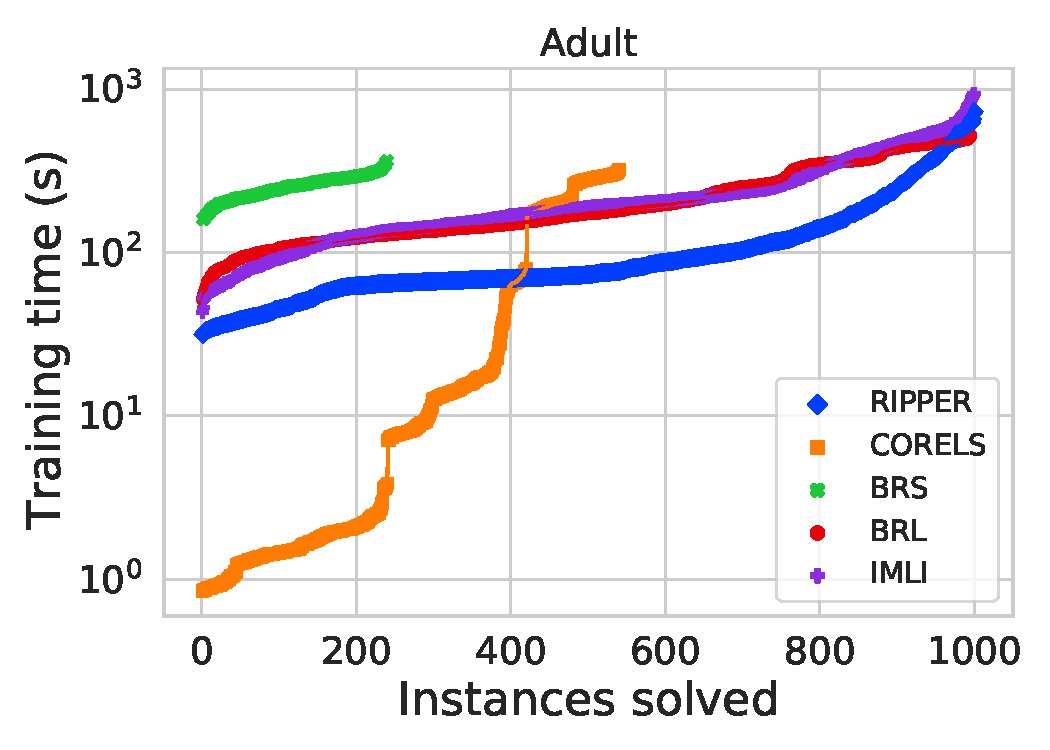
\includegraphics[scale=0.3]{figures/dataset_adult_cactus_train_val_fit_time}}
		\subfloat[Samples: $  107, 696 $\\Features: $ 169 $]{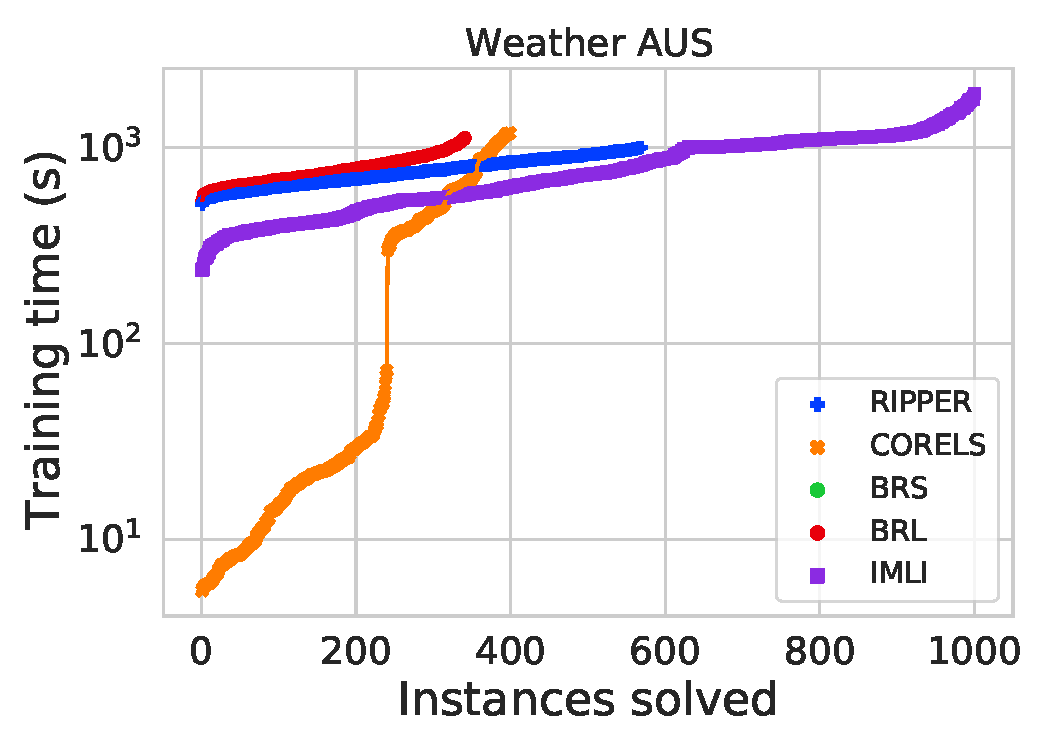
\includegraphics[scale=0.3]{figures/dataset_weatherAUS_cactus_train_val_fit_time}}
		\subfloat[Samples: $  1, 000, 000 $\\Features: $ 89 $]{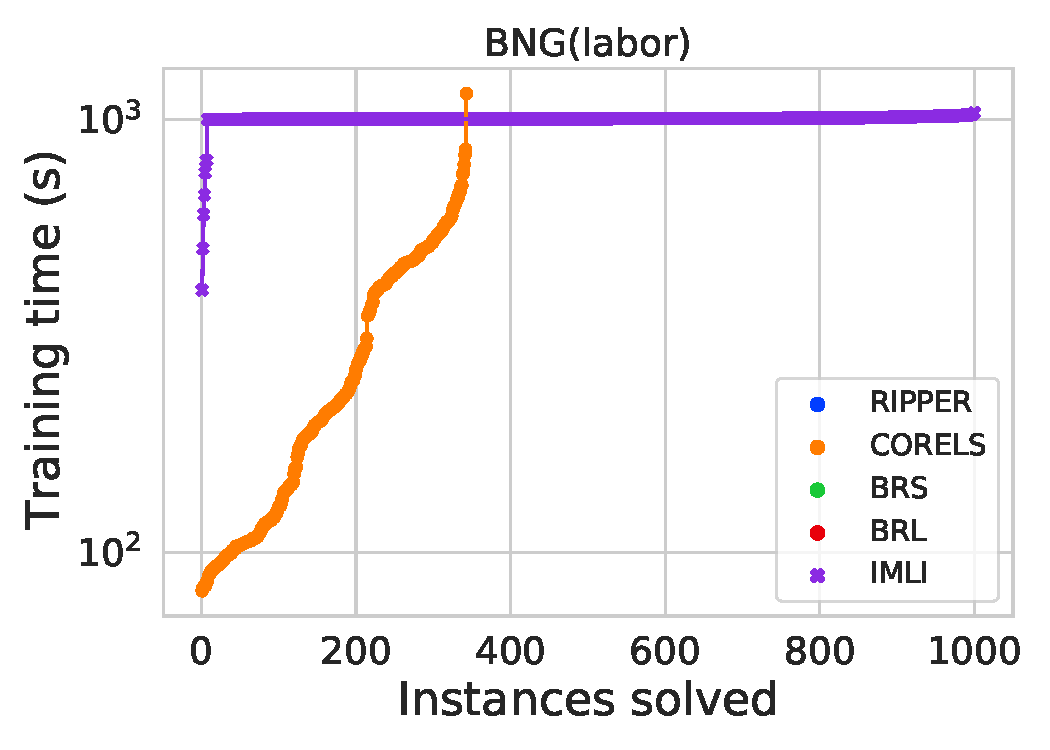
\includegraphics[scale=0.3]{figures/dataset_labor_cactus_train_val_fit_time}}
		
		\caption{Results on the scalability of $ \mathsf{IMLI} $ compared to existing interpretable classifiers, presented using cactus plots for datasets with varied dimensions. As datasets become large, $ \mathsf{IMLI} $ becomes the only interpretable classifier to classify all of $ 1000 $ classification instances for a dataset. The success of $ \mathsf{IMLI} $ is attributed to its incremental learning wrapping a MaxSAT-based formulation.}
		\label{fig:scalability_imli}
	\end{figure}
	\end{comment}
	
	
	
%	\paragraph{Classification Rules in Relaxed Logical Form.} We extend our incremental learning framework to learn a more relaxed representation of classification rules~\cite{ghosh2020classification}. Elaborately, we consider relaxed definitions of standard OR/AND operators in Boolean logic, which allow exceptions in the construction of a clause and also in the selection of clauses in a rule. Building on these relaxed definitions, we introduce relaxed-CNF classification rules motivated by the popular usage of checklists in the medical domain. Relaxed-CNF generalizes widely employed rule representations including CNF, DNF, and decision sets. While the combinatorial structure of relaxed-CNF rules offers exponential succinctness, the na\"ive learning techniques are computationally expensive. To this end, we propose an incremental mini-batch learning procedure, called $ \mathsf{CRR} $, that employs advances in the Mixed-Integer Linear Programming (MILP) solvers to efficiently learn relaxed-CNF rules. Our experimental analysis demonstrates that $ \mathsf{CRR} $ can generate relaxed-CNF rules, which are more accurate and sparser compared to the alternative rule-based models.
	
	

	
	\section*{Future Research Plans}
	 My long-term research plan is focused on designing efficient and scalable algorithms for machine learning, with a particular emphasis on their trustworthiness in safety-critical applications. To achieve this goal, I plan to work in a collaborative environment, where I can better understand the challenges arising in real-world applications and use advances in machine learning and formal methods to solve them. In pursuit of this vision, I have identified several key research themes that will guide my work.
	 
	 
	 \paragraph{Fairness and Interpretability As a Service.} I believe that in the future, machine learning will serve as an alternative decision-maker to humans in various domains, including law, education, and transportation. However, in high-stakes and safety-critical applications, black-box algorithms are expected to provide higher transparency. Therefore, it is crucial to achieve fairness, interpretability, robustness, and privacy in machine learning models. However, traditional machine learning models, such as deep learning, are often data-hungry, making it challenging to certify and verify properties such as fairness and interpretability in complex models and large datasets. With this in mind, my research aims to develop efficient algorithms for ensuring the fairness and interpretability of deep learning models, transformer-based natural language processing (NLP), and computer vision. 
	 
	 
	 \paragraph{Counting and Optimization Problems.} In my previous research, I focused on formulating fairness and interpretability in machine learning as counting and optimization problems. I developed algorithms based on formal methods and incremental solving, which resulted in both higher scalability and better accuracy. Building on this work, I plan to extend these techniques to solve counting and optimization problems in areas beyond machine learning.
	
	
	\bibliographystyle{ieeetr}		\bibliography{ref}
\end{document}